\documentclass[submit,techreq,noauthor]{eco}	% semi style
\usepackage[dvips]{graphicx}
\usepackage{listings, jlisting} 		% for source code
\usepackage[hyphens]{url}
\usepackage{setspace}
\usepackage{here}
\usepackage{xcolor}
%\setstretch{1.5} % 行間を広くします(資料チェックしてもらうときはコメントを外す)

% \lstset{
%   language={C},
%   basicstyle={\ttfamily},
%   identifierstyle={\small},
%   commentstyle=\color{black},
%   keywordstyle={\small\bfseries},
%   ndkeywordstyle={\small},
%   stringstyle={\small\ttfamily},
%   frame={tb},
%   breaklines=true,
%   columns=[l]{fullflexible},
%   numbers=left,
%   xrightmargin=0zw,
%   xleftmargin=3zw,
%   numberstyle={\scriptsize},
%   stepnumber=1,
%   numbersep=1zw,
%   lineskip=-0.5ex
%   breaklines=true,  % 行が長すぎる場合に折り返し
%   breakatwhitespace=true,  % 単語単位で折り返し
%   % commentstyle={\small\ttfamily \color[rgb]{0,0.5,0}},
%   % keywordstyle={\small\bfseries \color[rgb]{1,0,0}},
%   % stringstyle={\small\ttfamily \color[rgb]{0,0,1}},
% }

% C言語のソースコードを表示するための設定
\lstset{
  language=C,
  identifierstyle=\small,
  ndkeywordstyle=\small,
  basicstyle=\ttfamily\small,
  keywordstyle=\small\bfseries\color{blue},
  commentstyle=\color{green!60!black},
  stringstyle=\small\color{orange},
  numbers=left,
  numberstyle=\tiny,
  stepnumber=1,
  breaklines=true,  % 行が長すぎる場合に折り返し
  breakatwhitespace=true,  % 単語単位で折り返し
  frame=single,
  % backgroundcolor=\color{gray!10},
  tabsize=4,
  lineskip=-0.5ex,
  escapeinside={<latex>}{</latex>},
  xrightmargin=0zw,
  xleftmargin=3zw,
}

\begin{document}

\semino {5/45}					% 年度/回数
\date   {5/12/14/木}				% 令和/月/日/曜日
\title  {ELFバイナリ実行時の動的リンカ内の情報の取得と\\重複シンボルの検出の実装}	% タイトル
\author {奥 若菜}				% 氏名


\begin{abstract}
	Linuxマシンが製品やサービスの基盤として広く利用されるようになっていることで,それを標的とするLinuxマルウェアが劇的に増加している.
  また,Linuxマルウェアの開発動向として,マルウェアが自身の攻撃をセキュリティソフトに検知されないようにする検知回避技術の大幅な向上が確認されている.
  2021年に発見されたマルウェアSymbioteは,一般的に見られるLinuxマルウェアと比較して,極めて検出が困難とされる.
  SymbioteはLD\_PRELOADを使用して,すべての実行中のプロセスにロードされる共有ライブラリとして動作し,
  正当なプロセスの下で自身や他のマルウェアの痕跡を隠蔽する.
  このように,動的リンカの機能を利用して,悪意のある共有ライブラリをプロセスにロードさせる攻撃をDynamic Linker Hijackingという.
  本校では,動的リンカに着目して,マルウェアの検知を困難にするDynamic Linker Hijackingの対策を検討する.
  今回は,Dynamic Linker Hijackingの検出手法について検討した.
  % 今回は,ELFバイナリ実行時に,Dynamic Linker Hijackingの影響が現れる箇所をすべて明らかにし,動的リンカ内から影響に関する情報を取得できることを確認する.
  % さらに,ロードされるオブジェクト間でのシンボルの重複を検出する機能を動的リンカ内に実装する.
\end{abstract}
\maketitle


\section{はじめに}
  IoTデバイスの普及や組織のクラウドシフトにより,製品やサービスの基盤として,Linuxマシンを利用するケースが増えた.
  攻撃対象が広がったことで,それを標的とするLinuxマルウェアも劇的に増加している.
  AV-ATLASのマルウェアの統計データによると,Linuxを標的とした新種のマルウェアは2022年上半期に1,687,755個見つかっており,2021年上半期の226,324個と比較して,約650\%増加している\cite{AV-TEST}.
  Linuxマルウェアの動向としては,マルウェアが自身の攻撃をセキュリティソフトに検知されないようにする検知回避技術の大幅な向上が確認されている\cite{IBM}.
  このようなLinuxマルウェアとして,特にDynamic Linker Hijackingを行うマルウェアが注目されている.

  2021年に発見されたSymbiote\cite{Symbiote}は,動的リンカによって,実行中のプロセスにロードされる共有ライブラリとして動作する.
  攻撃者はLD\_PRELOADという環境変数を利用し,Symbioteを優先してロードさせることで,本来使用されるライブラリ関数を置き換える.
  Symbioteの検出が困難な理由として,ライブラリ関数の置き換えによって,正常なプロセスの下で任意のコードの実行が可能になることがある.
  これによって悪意のあるファイルやプロセス,通信の隠蔽や改ざんが行われる.
  このように,動的リンカの機能を利用して,悪意のある共有ライブラリをプロセスにロードさせる攻撃をDynamic Linker Hijackingという.

  Dynamic Linker Hijackingの対策として,動的リンカに関する環境変数や設定ファイルの変更を監視することが提案されている\cite{MITRE-ATT&CK}.
  この対策の目的は,攻撃者によって,プロセスにロードする共有オブジェクトの設定が行われるのを防ぐことである.
  しかし,この設定が行われてしまい,プロセスにマルウェアの共有オブジェクトがロードされる場合も,プロセスの実行時にロードを防ぐことが期待される.

  本稿では,共有オブジェクトのロードを行う動的リンカに着目し,プロセス実行時の動的リンク段階におけるDynamic Linker Hijackingへの対策を検討する.
  今回は,ELFバイナリ実行時に,Dynamic Linker Hijackingの影響が現れる箇所をすべて明らかにし,動的リンカ内から影響に関する情報を取得できることを確認する.
  さらに,ロードされる共有オブジェクト間でのシンボルの重複を検出する機能を動的リンカ内に実装する.
  % Dynamic Linker Hijackingは,マルウェアの検知を非常に困難にする.
  %正当なプロセスの下で,マルウェアのコードが実行されるため,プロセスベースの解析は回避される可能性が高い.

  以下,2章でDynamic Linker Hijacking検出のフックポイントについて述べ,3章で検出手法の概要を述べる.
  4章でLinuxのソフトウェアにおける動的リンク状況の調査について述べ,5章で検出における脅威度の判定方法について述べる.最後に6章でまとめる.\\


\section{Dynamic Linker Hijacking検出のフックポイント}
本章では,Dynamic Linker Hijackingの検出において,攻撃の可能性がある場合に,もれなく検査を行うためのフックポイントを示す.
Linuxの動的リンカの調査の結果,プロセスに任意の共有オブジェクトをロードさせる機能は以下の3つである.
\begin{itemize}
  \item 動的セクション DT\_RPATH,DT\_RUNPATH
  \item 環境変数 LD\_LIBRARY\_PATH
  \item 環境変数 LD\_PRELOAD,/etc/ld.so.preload
  %\item GNU gdb (Ubuntu 12.1-0ubuntu1~22.04) 12.1
 \end{itemize}

 DT\_RPATH,DT\_RUNPATHは,プログラムのコンパイル時に共有オブジェクトの検索パス指定することで,実行可能ファイルに検索パスを埋め込む.
 一方で,LD\_LIBRARY\_PATH,LD\_PRELOAD,/etc/ld.so.preloadはプログラムの実行時に共有オブジェクトや,共有オブジェクトの検索パスを追加する.

 Dynamic Linker Hijackingは,攻撃者によって実行可能ファイルが感染端末にインストールされる攻撃や,感染端末でプログラムがコンパイルされるような攻撃を含まない.
 よって,LD\_LIBRARY\_PATH,LD\_PRELOAD,ld.so.preloadのいずれかが使用されるときに攻撃の判定を行うことで,Dynamic Linker Hijackingによってロードされる共有オブジェクトを漏れなく検査することができる.\\


% \subsection{実験環境}
% 実験に用いる動的リンカと動作環境を以下に示す.
% \begin{itemize}
%   \item ld-linux-x86-64.so.2(glibc version 2.35)
%   \item Ubuntu 22.04.2 LTS
%   \item QEMU 6.2.0  
%   %\item GNU gdb (Ubuntu 12.1-0ubuntu1~22.04) 12.1
%  \end{itemize}

\section{検出手法の概要}
本章では,Dynamic Linker Hijackingの検出手法の概要について述べる.

\begin{figure*}[t]
	\centering
  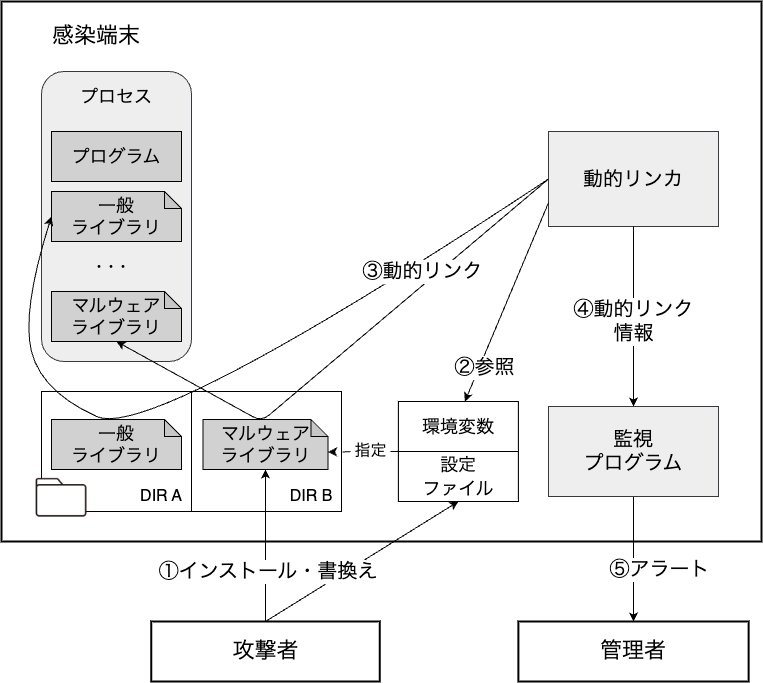
\includegraphics[width=13cm]{fig/method3.png}
	\caption{マルウェアなしの/usr/bin/sshのscope}
	\label{fig:method}
\end{figure*}



\subsection{オブジェクトのロード順・ロードパスの取得}
\subsubsection{scope}
ELFバイナリ実行時に,動的リンカがプロセスにロードする共有オブジェクトのロード順とロードパスは,動的リンカ内で管理されるscope配列から取得できる.
scopeはオブジェクトのリンクマップを格納する配列であり,1つのリンクマップは対応する1つのオブジェクトの情報を持つ.
動的リンカはシンボルの検索を行うときに,scopeに格納されたリンクマップの順にオブジェクトのシンボルテーブルを探索する.
プロセスにロードされたオブジェクトはそれぞれscopeを持つ.
動的リンカ本体のオブジェクト(ld-linux-x86-64.so.2)はscopeを持たないなど,特殊な場合を除いて各オブジェクトのscopeの中身は同じである.
よって,ここでは実行するELFバイナリのリンクマップであるmain\_mapのscopeを代表に用いる.

動的リンカのソースコードより,scopeは,プロセスにロードしたオブジェクトの順番にリンクマップを格納することが分かった.
%ただし,動的リンカのオブジェクトは,動的リンクを行うために,依存関係に関わらずロードされ,依存関係を持たない場合はscopeから除外される.
またリンクマップは,オブジェクトの完全パスの情報を持つ.
よって,main\_mapのscopeを確認することにより,プロセスにロードされるオブジェクトのロード順とロードパスを取得することができる.\\

\subsubsection{scopeの取得結果}

\begin{figure*}[t]
	\centering
  \includegraphics[width=13cm]{fig/scope1.eps}
	\caption{マルウェアなしの/usr/bin/sshのscope}
	\label{fig:scope}
\end{figure*}

\begin{figure*}[t]
	\centering
  \includegraphics[width=13cm]{fig/scope2.eps}
	\caption{マルウェアありの/usr/bin/sshのscope}
	\label{fig:scope-malware}
\end{figure*}

Dynamic Linker Hijackingによって,オブジェクトのロード順またはロードパスが変化することを,実際のELFバイナリを実行したときのscopeを取得することで確認した.
scopeの値は,動的リンカのデバッグを行う環境変数LD\_DEBUGにscopesを設定することで,実行時に動的リンカに出力させる.
実行するELFバイナリは/usr/bin/sshを用い,ssh localhostを実行したときの/usr/bin/sshのscopeを取得する.
条件として,LD\_PRELOADが値を持たないとき(マルウェアなし)と,Dynamic Linker Hijackingを想定して,
LD\_PRELOADにマルウェアの共有オブジェクトのパス/home/woku/Symbiote-20220610/kerneldev.soを設定したとき(マルウェアあり)で行う.

マルウェアなしとマルウェアありの結果を,それぞれ図\ref{fig:scope}と図\ref{fig:scope-malware}に示す.
両方の図にある水色マーカー部分は,どのオブジェクトのscopeであるかを表しており,/usr/bin/sshのscopeであることが分かる.
「scope 0:」の文字列以降は,scopeの中身であり,オブジェクトのパスが空白区切りで示されている.
図\ref{fig:scope}と図\ref{fig:scope-malware}のscopeを比較すると,図\ref{fig:scope-malware}の黄色マーカー部分のオブジェクトが,図\ref{fig:scope}には存在しないことが分かる.
追加されたオブジェクトは,LD\_PRELOADによって設定されたマルウェアのオブジェクトと,そのオブジェクトが依存する共有オブジェクトである.
この結果から,動的リンク時のscopeを取得することで,オブジェクトのロードパス,ロード順が分かり,
Dynamic Linker Hijackingが行われるときは,それらの変化が確認できることを示した.\\

\section{シンボル重複の検出}
\subsection{Dynamic Linker Hijackingにおけるシンボル重複}
動的リンカが行うシンボル解決では,ロードされたオブジェクト間にシンボルの重複あった場合,先にロードされたオブジェクトのシンボルが解決に使用される.
通常のシステムでは,特別な理由がない限り,重複シンボルは意図しない動作の原因となる可能性があるため,なくすべきとされる.
一方で,Dynamic Linker Hijackingでは,正規のライブラリと同名のライブラリを持つオブジェクトを優先的にロードさせ,シンボル重複を起こすことで,ライブラリの置き換えを行う.
よって,プロセスにロードされたオブジェクト間にシンボルの重複が存在する場合,Dynamic Linker Hijackingの可能性を疑うべきである.

\subsection{シンボル重複の検出機能の実装}
Dynamic Linker Hijackingの対策として,プロセスにロードされたオブジェクト間のシンボル重複を検出したい.
しかし,動的リンカの通常のシンボル解決では,目的のシンボルを発見した時点でシンボルの探索を終了するため,重複シンボルを検出できない.
そこで,動的リンカ内にシンボルの重複を検出するための機能を実装する.

重複シンボルの検出はなるべく早い段階でおこないたい.
よって,プロセスにオブジェクトが全てロードされた後,実際のシンボル解決処理の前に,シンボル重複の検出処理を追加する.\\

\subsubsection{シンボル重複の検出手法}
動的リンカのソースコードに,シンボル重複の検出を行う関数 \_dl\_detect\_duplicate()を追加した.
図\ref{listings:code}にソースコードを示し,以下に関数の処理の流れを説明する.

\begin{enumerate}
  \item 引数として,シンボル重複を探したいオブジェクトのリンクマップdef\_mapと,そのscopeを受け取る.
  \item def\_mapのシンボルテーブルと文字列テーブルのエントリアドレスを取得する.
  \item scopeの順番を変更し,def\_mapを一番最後に移す.
  \item シンボルテーブルの先頭からシンボルを順番に見ていく.
  \item シンボルの定義がUNDEFでないかつ,グローバルスコープなら,def\_mapのオブジェクトによって解決されるシンボルとみなす.
  \item def\_mapのオブジェクトによって解決されるシンボルなら,文字列テーブルからシンボル名を取得する.
  \item 動的リンカの関数\_dl\_lookup\_symbol\_xにシンボル名とスコープを渡して,def\_map以外からシンボルを探す.
  \item シンボルがdef\_map以外から見つかった場合,重複シンボルとして,定義しているオブジェクト2つとシンボル名を出力する.\\
\end{enumerate}

\subsubsection{実行結果}
\_dl\_detect\_duplicate()を動的リンカ内で呼び出すことによって,シンボルの重複が検出できることを確認する.
LD\_PRELOADにマルウェアの共有オブジェクトのパス/home/woku/Symbiote-20220610/kerneldev.soを設定し,usr/bin/lsを実行したときの出力を確認した.
出力結果を図4に示す.水色マーカーの部分のオブジェクトと,灰色マーカーの部分のオブジェクトで,fopenのシンボルが重複していることが分かる.
また,全部で6つのシンボルが検出されており,ロードされたオブジェクトから重複シンボルが全て検出できることを確認した.\\


\section{おわりに}
今回は,Dynamic Linker Hijackingの影響が現れる箇所をすべて明らかにし,動的リンカ内から影響に関する情報を取得できることを確認した.
また,プロセスにロードされたオブジェクト間のシンボルの重複を検出する機能を動的リンカ内に実装した.
今後は,実際のソフトウェアにおいて,これらの情報を調査する.
具体的には,Linux等における環境変数の利用具合や,オブジェクトの配置に使用されるディレクトリの確認などを行う.
得られた情報から,通常の状態と異常な状態を定義し,状態に合わせて具体的な対策を実施する.


\begin{figure*}[t]
	\centering
  \includegraphics[width=13cm]{fig/dup.eps}
	\caption{シンボル重複の検出結果}
	\label{fig:duplicate}
\end{figure*}



%bibtex
\setlength\baselineskip{12pt}
{\small
	\bibliography{references}
	\bibliographystyle{ipsjunsrt}
}

\end{document}
